\documentclass[a4paper,11pt]{article}

\pdfminorversion=4

\usepackage{cmap}
\usepackage[utf8]{inputenc}
\usepackage[T1]{fontenc}
\usepackage{lmodern}
\usepackage{geometry}
\usepackage{graphicx}
\usepackage{amsmath}
\usepackage{amssymb}
\usepackage{xcolor}
\usepackage{listings}
\usepackage{float}
\usepackage{hyperref}

\geometry{margin=2.4cm}
\setlength{\parindent}{0pt}
\setlength{\parskip}{0.65em}
\setlength{\emergencystretch}{2em}
\renewcommand{\abstractname}{Abstract}
\renewcommand{\figurename}{Figure}

\lstset{
  basicstyle=\ttfamily\small,
  breaklines=true,
  frame=none,
  backgroundcolor=\color{gray!8},
  xleftmargin=1em,
  xrightmargin=1em,
}

\title{Software Architecture as a Layered Representation\\
  \large Analyzing Software Architecture with S202}
\author{Johannes Weigend}
\date{Final version, May~26,~2026}

\begin{document}

\maketitle

\begin{abstract}
S202 computes a hierarchical layered representation of Java systems from
bytecode. The tool derives an architectural hypothesis from the observed class
dependencies, makes cycles and back edges visible as explicit findings, and
checks the finished representation redundantly against consistency rules. This
document describes typical errors in the computation of such layouts, explains
the conceptual solution, and shows how the representation can be used as a
working tool for refactoring planning.
\end{abstract}

\section{Introduction}

At least since the layered models for operating systems in the late 1960s,
software architecture has been represented as a layered dependency structure.
The principle is still relevant today: in cloud-native architectures it helps
to order technical dependencies between services, platforms, and
infrastructure; in domain-driven design it helps to make domain boundaries and
dependencies between bounded contexts visible. The basic idea is simple: an
element that uses another element is placed above the element it uses.
Dependencies therefore run from top to bottom. Edges in the opposite direction
stand out because they often indicate cycles, unwanted coupling, or a broken
layering order.

Such vertically aligned graphs help to understand systems and to detect
anomalies in their dependencies. A simple example is provided by the Java tool
\texttt{jdeps} and the Graphviz tool \texttt{dot}: \texttt{jdeps} extracts
class dependencies from a JAR, and \texttt{dot} turns them into a directed
graph.

\newpage

Figure~\ref{fig:acyclic-levels} shows an acyclic example from the Example JAR
of the S202 codebase. It was created with \texttt{jdeps} and \texttt{dot}. The
JAR contains nine classes in three packages: \texttt{example},
\texttt{example1}, and \texttt{example2}.

\begin{figure}[H]
  \centering
  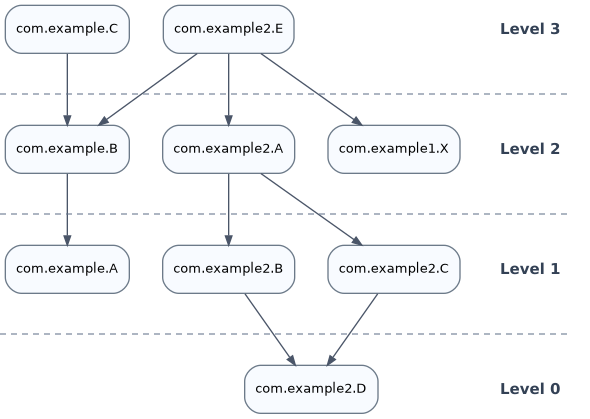
\includegraphics[width=0.75\textwidth]{figures/test-example-classgraph-acyclic-levels.png}
  \caption{Acyclic example from \texttt{test-example-1.0.0.jar}.}
  \label{fig:acyclic-levels}
\end{figure}

The arrows between the boxes are dependencies between classes by invocation or
use. In the example, \texttt{com.example.B} uses class
\texttt{com.example.A}, abbreviated as $B \to A$. The horizontal lines were
added manually and visualize the levels of the layering. Level~0 forms the
foundation; higher levels represent elements that depend on elements below
them.

This kind of representation is useful and widely used. As a visualization of
real applications, however, it has three practical problems:

\begin{enumerate}
  \item Many arrows make the graph hard to read even for medium-sized
        applications.
  \item The package structure is spread across several levels and does not
        form a visible grouping.
  \item With cyclic dependencies, the cycle must be broken for level
        computation so that any vertical order can be created at all. The
        original dependency graph remains unchanged; only the derived DAG
        (\emph{Directed Acyclic Graph}) used for level computation is changed.
        The decisive question is therefore which edge is excluded from this
        computation, because exactly this edge later appears as a break in the
        computed order.
\end{enumerate}

\section{S202 as a Hierarchical Layered Representation}

With the open source tool S202, we address these problems directly. S202 does
not simply replace the flat class graph with an improved representation. It
replaces it with a hierarchical architectural hypothesis: packages remain
visible as containers, and inside each container, packages or classes are
ordered by their dependencies.

The arrows can be shown optionally. In the normal case, however, the vertical
order alone should make it understandable which parts of the application are
higher up and which parts serve as the foundation. Unwanted dependencies
therefore do not appear merely as a single line in a large network, but as a
break in an expected layering order.

Unlike the flat class graph, S202 structures levels hierarchically through the
package structure. Each package orders its direct children, that is,
subpackages or classes, according to their local dependencies. The package
structure remains visible instead of being pulled apart by the class graph.

\begin{figure}[H]
  \centering
  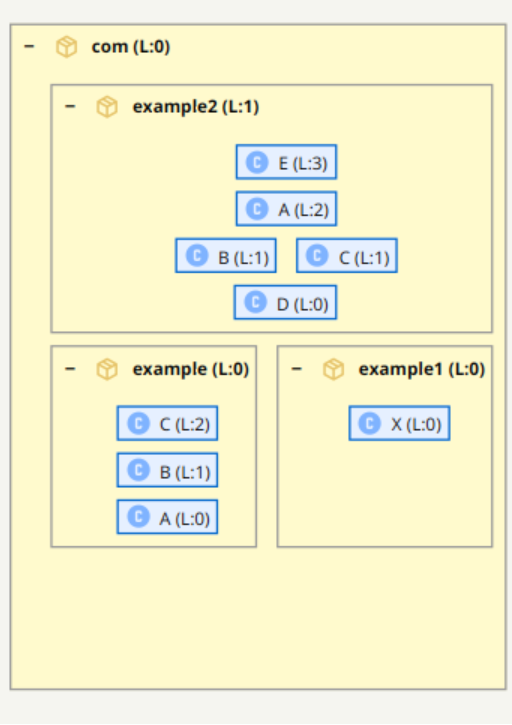
\includegraphics[width=0.55\textwidth]{figures/s202-dependencies-acyclic.png}
  \caption{S202 representation of the acyclic example: packages remain visible
  as containers, classes are ordered within their container, and arrows can be
  shown when needed.}
  \label{fig:s202-acyclic}
\end{figure}

The example shows the package structure below the outer package
\texttt{com}: \texttt{example}, \texttt{example1}, and \texttt{example2} are
subtrees of this container. In the \texttt{example2} subtree there is a
non-trivial internal class structure; at the same time, the overarching
structure shows that \texttt{example2} depends on \texttt{example} and
\texttt{example1}. At class level, \texttt{example2} has the order
$E \to A \to (B \mid C) \to D$. The representation deliberately abstracts
from individual edges. Whether \texttt{A} has a dependency to \texttt{B}, to
\texttt{C}, or to both is less important for the coarse architectural view
than the layering of the package. This abstraction is exactly what keeps large
relationship networks readable.

The idea is not new. The commercial product Structure101 already had a very
similar representation. However, there is no open implementation and no
technical documentation that explains how such a layout can be computed
reliably. S202 closes this gap as an open source tool under the Apache license.

This document describes the typical pitfalls in implementing such a layout and
shows a solution that eliminates many of these problems cleanly at the
conceptual level.

\section{Typical Errors in Computing Layers}

Figures~\ref{fig:acyclic-levels} and~\ref{fig:s202-acyclic} deliberately show
a simple, acyclic example. In this case the layering is unambiguous:
\texttt{E} is above \texttt{A}, \texttt{A} is above \texttt{B} and
\texttt{C}, and both are above \texttt{D}. There is no feedback, so no edge
has to be selected and ignored for level computation.

In real applications this case is the exception rather than the rule. As soon
as classes or packages depend on each other cyclically, a normal graph pass is
no longer sufficient. This is where the interesting errors begin: the
representation may still look plausible, but the computed levels are no longer
stable or no longer explainable in architectural terms.

In the following sections, the term SCC plays a central role. An SCC
(\emph{Strongly Connected Component}) is a set of nodes in which every node can
reach every other node through directed dependency paths. In such a cycle, not
all dependencies can run downward at the same time.

A correct layered layout must therefore satisfy several requirements at once:

\begin{enumerate}
  \item If $A \to B$, then $A$ must be placed above $B$.
  \item Packages must remain visible as containers. A package must not be moved
        accidentally just because a single contained class has a high class
        level.
  \item Classes or packages that form an SCC must be handled explicitly,
        because in a cycle not all edges can run downward at the same time.
\end{enumerate}

Each requirement is manageable in isolation. Together, however, they create a
circular dependency system between the levels of computation themselves: class
levels influence visible positions, package containers structure these
positions, and SCCs force corrections to an order that would already have been
computed without cycle handling. This is the source of the typical failure
modes.

\subsection{Retroactive Correction}

Retroactive correction means here that a structure discovered later forces a
subsequent change to levels that have already been computed.

A naive algorithm iterates over the classes and assigns levels directly. It
first sees class \texttt{A}, assigns its level, and thereby also lifts the
package of \texttt{A}. Later it finds class \texttt{B} and discovers that
\texttt{A} and \texttt{B} belong to the same SCC and must be handled together.
Now \texttt{A} would have to be corrected, and with it its package and possibly
further packages that depend on it.

The problem is not the correction itself. The problem is that parts of the
layout have already been treated as finished at that point. An algorithm that
mixes cycle detection and level assignment has to change, retroactively, places
that it had already left behind.

\subsection{Order-Dependent Results}

Classes come from JARs. The order in which a tool sees classes follows not the
architecture, but the packaging order of the JAR, the module order, the build
tool, or filesystem details. If an algorithm handles cycles as a side effect
during this traversal, the result depends on this accidental order.

This is dangerous because the error does not have to be immediately visible.
The graph may still look roughly correct. Nevertheless, the same codebase can
receive different levels depending on the build configuration.

\subsection{Mixed Class and Package Levels}

One obvious mistake is to derive the level of a package from the highest level
of the classes it contains. This sounds plausible, but it mixes two different
questions: where a class lies in the class graph, and where a package lies in
the architectural hypothesis.

A package is not architecturally high just because it happens to contain a
highly placed class. The central rule is:

\begin{quote}
  Package levels are derived from package dependencies, not from the maximum
  height of individual classes.
\end{quote}

This sounds trivial, but it is not. Precisely because packages are containers
for classes, it is tempting to derive their position from the classes they
contain. That is exactly how two levels get mixed that must remain separate.
Only when package levels are derived from package dependencies do packages
remain stable architectural units. Otherwise a single outlier class is enough
to lift the package to the wrong level and thereby make the container
unusable, even though that container is supposed to provide orientation.

\subsection{The Big Lake}

The formally clean answer to cycles is: all elements of an SCC receive the
same level. For small cycles this is acceptable. In real systems, however,
SCCs can become very large. Then hundreds or thousands of classes end up on
the same level. The layering disappears; what remains is a flat block.

The cycle is then correctly detected, but no longer usefully visualized. A tool
must therefore be able to break large SCCs. The decisive point is that the cut
edges must not disappear. They must remain visible, because they explain why
the computed order is only an architectural hypothesis.

\section{The Package Graph as an Architectural Hypothesis}

The solution chosen by S202 is to separate analysis, ordering, and
representation consistently. The class graph remains the raw model of the
actual dependencies. It is not changed merely because a layered representation
requires a DAG. Instead, S202 creates additional views from this graph: SCCs
for cycle detection, a weighted package graph for the architectural
hypothesis, and a hierarchical UI structure for the representation.

The term architectural hypothesis does not mean an asserted target
architecture. It means the actual architecture inferred from the observed
dependencies: the order that best fits the existing code and its dependencies
without hiding where this order is broken by cycles or back edges.

The package ordering is the central connecting element. It is not derived from
the highest class levels, but from aggregated package dependencies. This
separation is the decisive step: classes are ordered within their packages,
whereas packages are ordered by their own package relationships. This allows a
package to remain stable as a container even when individual classes inside it
are high or low. At the same time, the package ordering provides a criterion
for selecting back edges not arbitrarily, but as concrete violations of the
expected order.

Thus, the failure modes described above do not disappear because of one
algorithmic trick, but because the computation steps have clear
responsibilities: first dependencies are analyzed, then a plausible order is
determined, then the visible structure is built, and finally the result is
checked to see whether the representation satisfies its own claim.

\section{From Class Dependencies to Package Ordering}

In S202, the flat class graph is not the visible layout model. It is an
analysis artifact: it is used to capture concrete dependencies, detect SCCs,
aggregate class dependencies into package relationships, and derive the later
levels from them. The visible S202 graph is then built from the package
structure and the local order inside package containers.

Package ordering is created locally in the context of a parent package. S202
does not compare arbitrary packages globally; it compares the direct child
packages of the same container. Classes are not comparison nodes in this step.
They provide the information for aggregation: a class dependency is rolled up
to the child packages in whose subtrees source and target are located.

For each parent package, S202 therefore creates a weighted sibling graph of its
child packages. The edges in this graph are directly observed package
dependencies between these child packages. If a class in the subtree of child
package $P$ uses a class in the subtree of child package $Q$, an edge
$P \to Q$ is created. Its weight is the number of concrete uses that are
rolled up to this package edge; for structural dependencies without invocation
counts, a weight of~1 is used. The opposite direction is counted as well.

The sibling graph contains only such direct package dependencies. From
$B \to A$ and $C \to B$, no additional edge $C \to A$ is created. The
transitive order emerges only in the subsequent level computation.
Dependencies within the same child package do not change the order of the
child packages; dependencies that leave the parent container are handled at a
higher level of the package structure. This comparison is repeated recursively
for all package containers. The ordering of classes inside a package container
is a subsequent step.

Before level computation, the sibling graph must be acyclic. If child packages
form an SCC, S202 uses a rank measure to evaluate whether a child package in
the current sibling graph tends more to use other packages or to be used by
them:

\[
  rank(P) = \frac{out(P) - in(P)}{\max(1,\; out(P) + in(P))}
\]

$out(P)$ is the sum of the edge weights from $P$ to other considered siblings
in the current graph, and $in(P)$ is the sum of the edge weights from these
siblings to $P$. A positive rank means that the package uses more than it is
used; it therefore tends to belong higher up. A negative rank means that the
package is more often used and tends to belong lower down.

In a package SCC, an edge $P \to Q$ is treated as a back edge only if
$rank(P)$ is lower than $rank(Q)$ by more than a threshold $\varepsilon$.
S202 currently uses $\varepsilon = 0.1$ for this. If two packages are too close
to each other, they conceptually remain peers and therefore stay on the same
level. A reciprocal invocation ratio of $100 : 101$ is therefore not a robust
architectural decision.

After this cycle handling, S202 computes levels on the resulting DAG. Level~0
contains the packages that do not use any other child packages in the current
computation graph. Every other package is placed one level above the highest
package it directly uses. This creates the transitive layering: from
$B \to A$ and $C \to B$, it follows that $A$ is on Level~0, $B$ on Level~1,
and $C$ on Level~2, even though no direct edge $C \to A$ exists.

\section{From Class Cycles to Package Ordering}

Figure~\ref{fig:cyclic-class} shows a cyclic example from the Example JAR as a
classic class graph. The two subgraphs for Notification and Payment each
contain feedback.

\begin{figure}[H]
  \centering
  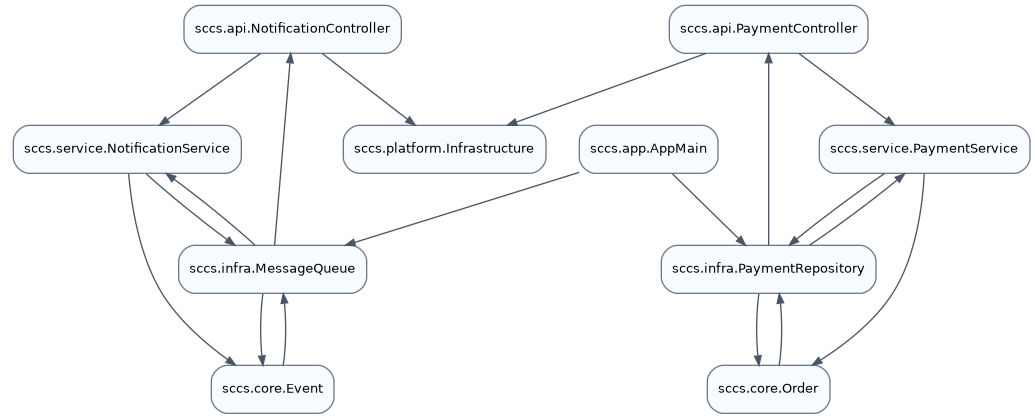
\includegraphics[width=0.9\textwidth]{figures/test-example-classgraph-cyclic.png}
  \caption{Cyclic example from \texttt{test-example-1.0.0.jar}. In every cycle,
  at least one edge must be cut for level computation.}
  \label{fig:cyclic-class}
\end{figure}

The marked cyclic areas are two non-trivial SCCs: one in the Notification part
of the example, with controller, service, message queue, and event classes, and
one in the Payment part, with controller, service, repository, and order
classes. The established procedure for finding such components is Tarjan's
algorithm.

In the cyclic case, the class graph therefore raises the technical question:
which edge must be ignored so that the SCC becomes a computable DAG again for
level assignment? The class graph alone does not provide an architectural
criterion for that. Only the package ordering provides this criterion: an edge
classified as a back edge is then not an arbitrary cut edge in the flat class
graph, but a concrete dependency that runs against the computed package order
and thereby makes the break in the architectural hypothesis visible.

\begin{figure}[H]
  \centering
  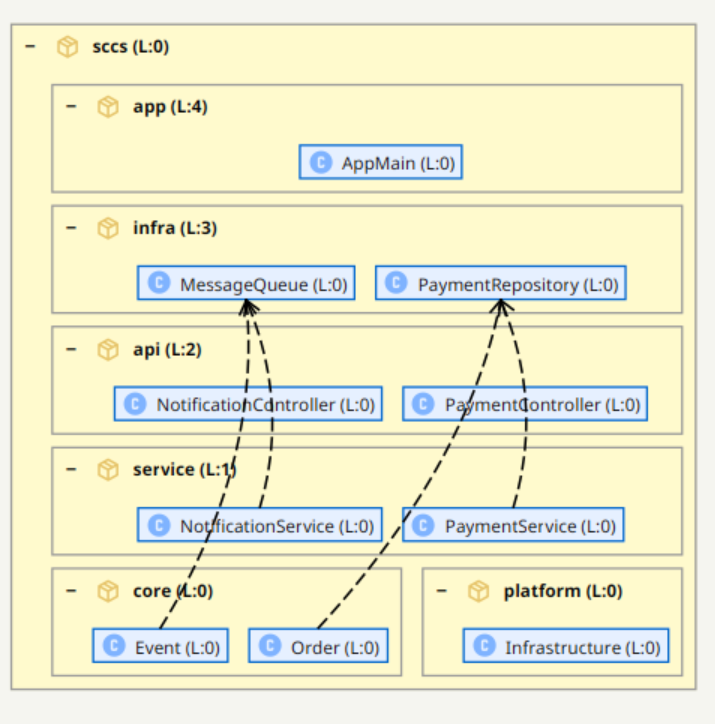
\includegraphics[width=0.6\textwidth]{figures/s202-dependencies-cyclic.png}
  \caption{Cyclic example in the S202 representation. The dashed edges are
  violations: they run against the order derived from package dependencies and
  remain visible findings of the architectural hypothesis. All four dashed
  edges belong to the two SCCs and are classified by S202 as back edges for
  level computation.}
  \label{fig:s202-cyclic}
\end{figure}

The terms back edge and violation describe different roles:

\begin{description}
  \item[Back edge] A selected edge inside an SCC that is handled separately for
        level computation so that the computation graph becomes acyclic. It
        belongs to cycle handling.
  \item[Violation] A concrete dependency that runs upward after the computed
        order has been applied. It may come from an SCC, but it does not have
        to. Violations are therefore a superset of back edges: a back edge can
        become visible as a violation, but not every violation is a back edge.
        Conceptually, a violation remains the visible deviation from the
        ordering, while a back edge describes the role of the edge in cycle
        handling.
\end{description}

S202 therefore does not hide the cycle. Edges classified as back edges remain
visible as violations because they explain why the package ordering does not
fully match the concrete class dependencies. This makes the deviation
traceable rather than arbitrary.

\section{Redundant Consistency Checking}

The steps described so far already show why the implementation is prone to
errors. It is not enough to secure individual algorithms with isolated unit
tests. Many errors arise only from the interaction of the data: concrete class
dependencies, package structure, SCCs, aggregated package weights, and local
layout positions influence one another.

S202 therefore checks more than individual computation steps. After the full
pipeline has run, the finished result is checked redundantly against
consistency rules. These rules do not recompute the layout and do not correct
anything. They only read the result and ask whether the generated
representation is internally consistent.

The check considers three levels:

\begin{enumerate}
  \item \textbf{Class graph:} For normal class dependencies, the following
        must hold: if $A \to B$, then $A$ is on a higher level than $B$.
        Exceptions must be classified explicitly, for example as a back edge
        or as an edge inside an SCC.
  \item \textbf{Package graph:} The computed package ordering must fit the
        weighted package dependencies. Packages with a higher rank must be
        above the packages on which they depend more strongly. Edges cut when
        breaking a package SCC must not be treated like normal dominant edges
        in this check; they must be classified separately as package back
        edges.
  \item \textbf{Visible representation:} The visible arrangement must match
        the computed model. Package containers, local class positions, and
        nested levels must not silently reverse the computed architectural
        hypothesis.
\end{enumerate}

These consistency rules are neither an additional optimization nor a second
layout algorithm. They are an independent plausibility check after the
calculation has finished. This is exactly why they find errors that normal
unit tests easily miss: a package level was computed correctly, but displayed
incorrectly locally; a back edge was cut, but not marked as such; a normal edge
runs upward without being part of an SCC.

The decisive point is redundancy. The pipeline generates the representation.
The rules then check whether this representation satisfies its own claim. This
turns a mere graphic into a verifiable model.

\section{From Visualization to Action}

A computed architectural hypothesis is especially useful when it does not only
describe a state, but also makes change plannable. S202 contains a what-if
analysis for this purpose: classes and packages can be moved in the
representation by drag and drop. The model is not refactored immediately;
instead, the tool computes which dependencies would run upward in the new
arrangement.

The violations are updated after every move. This shows whether a planned
reordering makes the architecture more consistent or introduces new problems.
This is especially important in situations where the tool can no longer find a
unique order: large SCCs, symmetric package dependencies, or historically grown
couplings cannot always be resolved automatically in a meaningful way.

\begin{figure}[H]
  \centering
  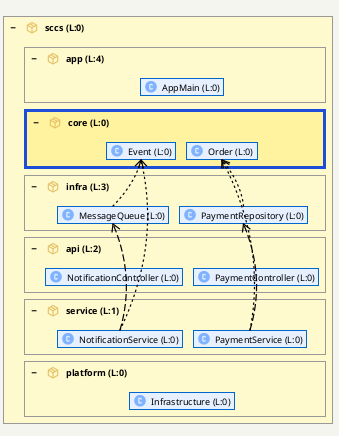
\includegraphics[width=0.45\textwidth]{figures/whatif-core-over-infra.png}
  \caption{What-if move: package \texttt{core} is moved from Level~0 between
  Level~3 and Level~4. This creates six violations because existing
  dependencies now run against the chosen arrangement.}
  \label{fig:whatif-core-over-infra}
\end{figure}

Figure~\ref{fig:whatif-core-over-infra} shows exactly this workflow: the manual
arrangement no longer corresponds to the order computed from the dependencies.
It can nevertheless express a desired target architecture, for example if
\texttt{core} should conceptually lie above the infrastructure. S202 therefore
does not treat this decision as an error in the representation, but makes its
cost visible: in this case, six concrete relationships would have to be
refactored or decoupled so that the dependencies again fit the chosen layering.

In addition, there is a manual CUT logic. Back edges can be marked deliberately
as planned cuts, and the tool can then check whether these cuts actually
resolve the affected SCC. The user not only sees which edge would be a
plausible break in the order, but can also verify the effect of that cut on the
cycle.

This CUT logic is more fine-grained than the visible class or package edge.
The cut is made at method-call level: not necessarily the entire relationship
between two classes disappears, but the concrete method call that causes the
cyclic dependency. This makes the feature fit practical refactoring work more
closely, because a cycle often arises from a few concrete calls, not from the
entire domain relationship between two classes.

\section{Implementation at the Conceptual Level}

The implementation deliberately separates the calculation into several phases.
The decisive point is that no phase fixes a visible position before the
information that justifies this position is available.

\begin{enumerate}
  \item \textbf{Build the class graph:} A directed class graph is created from
        the bytecode. This graph remains the domain raw model of the analysis.
  \item \textbf{Detect SCCs:} Strongly connected components are determined on
        the class graph using Tarjan. The result is not yet a layout; it is the
        information which classes can be ordered acyclically and which belong
        to cycles.
  \item \textbf{Derive the package graph:} Package dependencies are aggregated
        and weighted from the class dependencies.
  \item \textbf{Compute package ordering:} The rank measure $rank(P)$ is
        computed from the weighted incoming and outgoing edges. This yields the
        vertical package order. Small rank differences are treated as peer
        relationships.
  \item \textbf{Determine back edges:} Within each SCC, the edges sufficient
        for cycle removal are selected. These edges are back edges for level
        computation and remain visible as violations if they run upward after
        the computed order has been applied. Here, \emph{cut} does not mean
        that the edge disappears from the model. It is only excluded from the
        DAG used for level computation and remains preserved as a finding.
  \item \textbf{Build local layering:} Only after that is the visible tree
        structure created. Inside each container, only the direct children are
        ordered. This prevents the global package order from being mixed with
        local class levels.
  \item \textbf{Check consistency:} Finally, the finished representation is
        checked redundantly against the consistency rules. Normal dependencies,
        SCCs, back edges, and violations are distinguished and classified.
\end{enumerate}

In short:

\begin{lstlisting}
Bytecode -> class graph -> SCCs -> package graph -> package ordering
         -> back edges -> visible layering -> consistency rules
\end{lstlisting}

\section{Conclusion}

S202 computes the most plausible hypothesis of the actual architecture from
the existing dependencies. The result is a verifiable hierarchical layered
representation: class dependencies provide the graph, package dependencies
provide a robust order, back edges make necessary breaks visible, and
consistency rules check whether the finished representation satisfies its own
claim.

The most important contribution is therefore not an optically improved graph,
but the connection of representation, explanation, and changeability. The
layering shows a possible order. The marked findings explain where this order
is broken by concrete dependencies. What-if moves and manual CUTs make visible
which refactorings can reduce these breaks or actually dissolve cycles.

This makes the visualization more than a layout. It is an explainable working
model: every position and every highlighted edge must be traceable to a
comprehensible decision in the computation, and every planned change can be
checked against the same order.

\end{document}
